% Suggested LaTeX style template for Masters project report submitted at the
% Department of Computer Science and Technology
%
% Markus Kuhn, May 2022
% (borrowing elements from an earlier template by Steven Hand)

\documentclass[12pt,a4paper,twoside]{report}
% append option ",openright" after "twoside" if you prefer each chapter
% to start on a recto (odd-numbered) page in a double-sided printout

\usepackage[pdfborder={0 0 0}]{hyperref}  % turns references into hyperlinks
\usepackage[vmargin=20mm,hmargin=25mm]{geometry}  % adjust page margins
\usepackage{graphicx} % allows inclusion of PDF, PNG and JPG images
\usepackage{parskip}  % separate paragraphs with vertical space
                      % instead of indenting their first line
\usepackage{setspace} % for \onehalfspacing
\usepackage{refcount} % for counting pages
\usepackage{upquote}  % for correct quotation marks in verbatim text

\usepackage{courier}                  % better listings font
\usepackage{dirtytalk}                % quotations
\usepackage[square,numbers]{natbib}   % citations
\usepackage[chapter]{minted}          % code listings
\usepackage{multirow}                 % multi-row cells in tables
\usepackage{makecell}                 % multi-line cells in tables
\usepackage[subpreambles]{standalone}  % tex files as diagrams

% TODO: remove me
\usepackage{todonotes}
\setuptodonotes{inline}

\setminted{fontsize=\footnotesize,frame=lines,stripnl=false}

\newif\ifsubmission % Boolean flag for distinguishing submitted/final version

% Change the following lines to your own project title, name, college, course
\title{Void Processes: Minimising privilege by default}
\author{Jake Hillion}
\date{June 2022}
\newcommand{\candidatenumber}{2373A}
\newcommand{\college}{Queens' College}
\newcommand{\course}{Computer Science Tripos, Part III}
%\newcommand{\course}{Master of Philosophy in Advanced Computer Science}

% Select which version this is:
% For the (anonymous) submission (without your name or acknowledgements)
% uncomment the following line (or let the makefile do this for you)
%\submissiontrue
% For the final version (with your name) leave the above commented.

\begin{document}
%TC:ignore               % don't start counting words yet

\begin{sffamily} % use a sans-serif font for the pro-forma cover sheet

\begin{titlepage}
\makeatletter

% University logo with shield hanging in left margin
\hspace*{-14mm}
\includegraphics[width=65mm]{logo-dcst-colour}

\ifsubmission

% submission proforma cover page for blind marking
\begin{Large}
\vspace{20mm}
Research project report title page

\vspace{35mm}
Candidate \candidatenumber

\vspace{42mm}
\textsl{``\@title''}

\end{Large}

\else

% regular cover page
\begin{center}
\Huge
\vspace{\fill}

\@title
\vspace{\fill}

\@author
\vspace{10mm}

\Large
\college
\vspace{\fill}

\@date
\vspace{\fill}

\end{center}

\fi

\vspace{\fill}
\begin{center}
Submitted in partial fulfillment of the requirements for the\\
\course
\end{center}

\makeatother
\end{titlepage}

\newpage

Total page count: \pageref{lastpage}

% calculate number of pages from
% \label{firstcontentpage} to \label{lastcontentpage} inclusive
\makeatletter
\@tempcnta=\getpagerefnumber{lastcontentpage}\relax%
\advance\@tempcnta by -\getpagerefnumber{firstcontentpage}%
\advance\@tempcnta by 1%
\xdef\contentpages{\the\@tempcnta}%
\makeatother

Main chapters (excluding front-matter, references and appendix):
\contentpages~pages
(pp~\pageref{firstcontentpage}--\pageref{lastcontentpage})

Main chapters word count: 8291

Methodology used to generate that word count:

\begin{quote}
\begin{verbatim}
£ texcount report.tex | grep Words
Words in text: 8070
Words in headers: 93
Words outside text (captions, etc.): 128
\end{verbatim}

\texttt{texcount} macros are used to ensure counting begins on the first content page and ends on the last content page.
\end{quote}

\end{sffamily}

\onehalfspacing

\chapter*{Abstract}

The important of privilege separation - separating the parts of an application with the most risk of attack from the parts with the most reward for an attacker - for protection of resources in a modern operating system cannot be understated. As Linux has grown into the behemoth of an operating system that it is today, many privileges and attack vectors have been enabled, large amounts of which are given passively to new processes. New methods for protecting applications and processes have come along at nearly the same rate. This paper presents void processes: a framework to restrict Linux processes, removing access to ambient resources by default and providing APIs to systematically unlock abilities that applications require. Void processes solve the problem of needing to know what your privilege is in order to reduce it, as an application developer can begin from a clean slate.

This project built a system, the void orchestrator, to enable application developers to build upwards from a point of zero-privilege, rather than removing privilege that they don't need. This report gives the background and technical details of how to achieve this on modern Linux. I present a summary of the privilege separation techniques currently employed in production and details on how to create an empty set of namespaces to remove all privilege in Linux, a technique named entering the void. The shortcomings of Linux when creating empty namespaces are discussed, before setting forth the methods for re-adding features in each of these domains. Finally, two example applications are built and their performance evaluated to show the utility of the system. This report aims to demonstrate the value of a paradigm shift from reducing an arbitrary amount of privilege to adding only what is necessary.

\ifsubmission\else
% not included in submission for blind marking:

\chapter*{Acknowledgements}

This project would not have been possible without the wonderful
support of \ldots [optional]

\fi
\cleardoublepage % preserve page numbers after missing acknowledgements

\setcounter{tocdepth}{1} % only show up to sections in the table of contents
\tableofcontents
%\listoffigures
%\listoftables
%\lstlistoflistings


\chapter{Introduction}
\label{firstcontentpage} % start page count here
%TC:endignore            % start word count here
\label{chap:introduction}

Newly spawned processes on modern Linux are exposed to a myriad of attack vectors and privilege, whether the hundreds of system calls available, \texttt{procfs}, exposure of filesystem objects, or the ability to connect to arbitrary hosts on the Internet. This paper presents void processes: a framework to restrict Linux processes, removing access to ambient resources by default and providing APIs to systematically unlock abilities that applications require. Explicit privilege designation with void processes could have saved many applications from the threat of CVE-2021-44228 with Log4j2 by ensuring that the processes which do dangerous user data processing are sufficiently deprivileged to prevent remote code execution (§\ref{lst:fibonacci-application-spec}). Moreover, adding explicit privilege with each change encourages consideration of privilege separation whenever new privilege is added, rather than when flaws are exposed.

This project built a system, the void orchestrator, to enable application developers to build upwards from a point of zero-privilege, rather than removing privilege that they don't need. This report gives the background and technical details of how to achieve this on modern Linux. I present a summary of the privilege separation techniques currently employed in production (§\ref{chap:priv-sep}) and details on how to create an empty set of namespaces to remove all privilege in Linux (§\ref{chap:entering-the-void}), a technique named entering the void. The shortcomings of Linux when creating empty namespaces are discussed (§\ref{sec:voiding-mount},§\ref{sec:voiding-user},§\ref{sec:voiding-cgroup}), before setting forth the methods for re-adding features in each of these domains (§\ref{chap:filling-the-void}). Finally, two example applications are built (§\ref{chap:building-apps}) and evaluated (§\ref{chap:evaluation}) to show the utility of the system. This report aims to demonstrate the value of a paradigm shift from reducing an arbitrary amount of privilege to adding only what is necessary.

Much prior work exists in the space of privilege separation, including: virtual machines (§\ref{sec:priv-sep-another-machine}); containers (§\ref{sec:priv-sep-perspective}); object capabilities (§\ref{sec:priv-sep-ownership}); unikernels; and applications which run directly on a Linux host, potentially employing privilege separation of their own (§\ref{sec:priv-sep-process}, §\ref{sec:priv-sep-time}). These alternative environments are plotted in Figure \ref{fig:attack-vs-changes}, in which the difference between applications written for the environment and the attack surface remaining are compared. Void processes contribute a strong compromise between providing a rich Linux-like interface for applications, reducing necessary code changes, and significantly reducing the attack surface (demonstrated in §\ref{chap:entering-the-void}).

\begin{figure}[h]
    \centering
    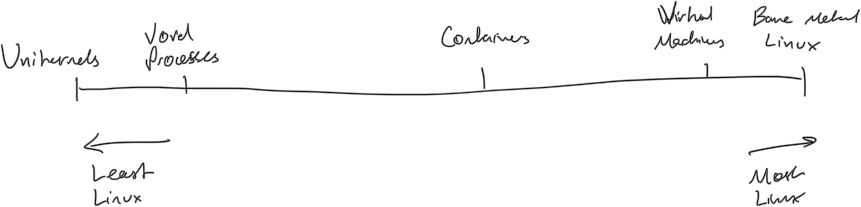
\includegraphics[width=0.6\textwidth]{figures/least-most-linux.png}
    
    \caption{Privilege separated environments plotted to compare the number of application changes required against the remaining attack surface of the environment.}
    \label{fig:attack-vs-changes}
\end{figure}


\chapter{Privilege Separation}
\label{chap:priv-sep}

Many attack vectors exist in software, notably in argument processing and deserialisation \citep{the_mitre_corporation_deserialization_2006,the_mitre_corporation_improper_2006}. Creating security conscious applications requires one of two things: creating applications without security bugs, or separating the parts of the application with the potential to cause damage from the parts most likely to contain bugs. Though many efforts have been made to create correct applications [CN], the use of such technology is far from widespread and security related bugs in applications are still frequent [CN]. Rather than attempting to avoid bugs, the commonly employed solution is privilege separation: ensuring that the privileged portion of the application is separated from the portion which is likely to be attacked, and that the interface between them is correct. This chapter details what privilege separation is, why it is useful, and a summary of some of the privilege separation techniques available in modern Unices. Many of these techniques are included in some form in the final design for void processes.

\section{Privilege separation by process}
\label{sec:priv-sep-process}

The basic unit of privilege separation on Unix is a process. If it's possible for an attacker to gain remote code execution in a process, the attacker gains access to all of that process's privilege. Reducing the privilege of a process therefore reduces the benefit of attacking that process. One solution to reducing privilege in the process is to take a previously monolithic application and split it into multiple smaller processes. Consider a TLS supporting web server that must have access to the certificate's private keys and also process user requests. These elements can be split into different processes. This means that if the user data handling process is compromised the attacker cannot access the contents of the private keys.

Application design in this paradigm is similar to that of a distributed system, where multiple asynchronous systems must interact over various communication channels. As an application becomes more like a networked system, serialisation and deserialisation becomes a common occurrence. As deserialisation is a very common source of exploits \citep{the_mitre_corporation_deserialization_2006}, this adds the potential for new flaws in the application.

OpenBSD is a UNIX operating system with an emphasis on security. A recent bug in OpenBSD's \texttt{sshd} highlights the utility of privilege separation \citep{the_openbsd_foundation_openssh_2022}. An integer overflow in the pre-authentication logic of the SSH daemon allowed a motivated attacker to exploit incorrect logic paths and gain access without authentication. Privilege separation ensures that the process with this bug, the pre-authentication process, is separated from the process which is able to be exploited, the highly privileged daemon. Moreover, privilege separation being mandatory in the software ensures that bugs which are not exploitable due to the privilege separation monitor's checks are not exploitable anywhere.

In 2003, privilege separation was added to the \texttt{syslogd} daemon of OpenBSD \citep{madhavapeddy_privsepc_2003}. The system is designed with a parent process that retains privilege and a network accepting child process that goes through a series of states, dropping privilege with each state change. This pattern allowed for restarting of the service while keeping the section which processed user data strongly separated from the process which remains privileged, by enabling the child process to cause its own restart while not holding enough privilege to execute that restart itself. An overview of the data flow is provided in Figure \ref{fig:openbsd-syslogd-privsep}.

\begin{figure}
    \centering
    \includestandalone[width=0.4\textwidth]{diagrams/openbsd-syslogd-privsep}
    
    \caption{Separation of privileged access from untrusted user data in OpenBSD's privilege separated syslogd design compared to the previous. The process which handles untrusted data is separated from the privileged process and uses RPC to communicate.}
    \label{fig:openbsd-syslogd-privsep}
\end{figure}

\section{Privilege separation by time}
\label{sec:priv-sep-time}

Many applications can privilege separate by using a single process which reduces its level of privilege as the application makes progress. This is effectively privilege separation over time. The approach is commonly to begin with high privilege for opening, for example, a listening socket below port 1000. After this has been completed, the ability to do so is dropped. One of the simplest ways to do this is to change user using \texttt{setuid(2)} after the privileged requirements are complete. An API such as OpenBSD's \texttt{pledge(2)} allows only a pre-specified set of system calls after the call to \texttt{pledge(2)}. A final alternative is to drop explicit capabilities on Linux. Each of these solutions irreversibly reduce the privilege of the process, known as dropping privilege. As the privilege has been irreversibly dropped, any attacker who gains control after the privilege has been dropped cannot take advantage of it.

After dropping privilege, it becomes difficult to do things such as reloading the configuration. The application process no longer has the required privilege to restart the application, and if it could gain it back then dropping it would have had no effect. This avoids having to treat the application as a distributed system as there continues to be only a single process to manage, which is often an easier paradigm to work in. The difficulty in implementing privilege dropping is ensuring that you know what privilege you hold, and drop it as soon as it is no longer required.

\section{Privilege separation by ownership}
\label{sec:priv-sep-ownership}

The previous methods shown each suffer from having to know what their initial privilege is in order to correctly deprivilege. An alternative method to enable the principle of least privilege in applications are object capabilities. An object capability is an unforgeable token of authority to perform some particular set of actions on some particular object.

While the methods looked at until now of privilege separation by process and time are supported by all Unices, object capabilities are a more niche system. Capsicum added object capabilities and was included in FreeBSD 10, released in January 2014 \citep{watson_capsicum_2010}. These capabilities may be shared between processes as with file descriptors. Capability mode removes access to all global namespaces from a process, allowing only operations on capabilities to continue. These capabilities are commonly those opened before the switch to capability mode, but they can also be sent and received (as file descriptors) or converted from a capability with more privilege to a capability with less.

Although object capabilities still require some additional work to ensure that only intentional capabilities remain accessible when entering capability mode, they come a lot closer to easy deprivileging than the previous solutions. However, their adoption remains limited at this point. They are unavailable in the latest Linux kernel release (5.17.7) at the time of writing, and there are no plans for their adoption.

\section{Privilege separation by using another machine}
\label{sec:priv-sep-another-machine}

One of the older methods of privilege separation is placing parts of an application on entirely different machines. If developing a web application, one might place the PHP backend on one machine and the database server on another. This means that even if a bad actor achieves remote access to the exposed PHP backend, they can only access the database server over its exposed API on the network, rather than having control of the machine itself. This allows features such as the database's access control to remain working, limiting the potential damange of an attacker controlling the PHP server.

Virtual machines \citep{barham_xen_2003,vmware_inc_understanding_2008} made the separation of privilege by machine a much more optimal use of hardware. Rather than requiring two full servers, one might instead provide both the application backend and the database server on a single physical machine but different virtual machines. This increased hardware usage in a time when hardware speed seemed in excess, and provided very strong isolation (presuming one couldn't escape the hypervisor). Though the isolation is strong, there are overheads associated with full virtualisation, and a more performant solution was sought.

\section{Privilege separation by perspective}
\label{sec:priv-sep-perspective}

Linux approaches increased process separation using namespaces. Namespaces control the view of the world that a process sees. Processes remain the primary method of separation, but utilise namespaces to increase the separation between them. The intended and most common use case of namespaces is providing containers. Containers approximate virtual machines, providing the appearance of running on an isolated system while sharing the same host. Containers, however, have to implement privilege separation in a very different way to the privilege separation we've seen previously. Rather than spawning multiple processes and employing privilege separation techniques to limit the attack vector in each, one spawns multiple containers to form a more literal distributed system. It is common to see, for example, a web server and the database that backs it deployed as two separate containers. These separate containers interact entirely over the network. This means that if a user achieves remote code execution of the database, it does not extend to the web server. This presents an interesting paradigm of small applications which can and often do run on separate physical hosts combining to provide a unified application experience.

\section{Summary}

This work focuses on the application of namespaces to more conventional privilege separation. Working with a shim which orchestrates the process and namespace layout, Void Applications seek to provide a completely pruned minimal Linux experience to each void process within the application. This builds on much of the prior work to severely limit the access of processes in the application. There is never a need to drop privileges as processes are created with the absolute minimum privilege necessary to perform correctly. In Chapter \ref{chap:entering-the-void} we discuss each namespace's role in Linux and how to create one which is empty, before explaining in Chapter \ref{chap:filling-the-void} how to reinsert just enough Linux for each process in an application to be able to complete useful work. These combine to form an architecture which minimises privilege by default, motivating highly intentional privilege separation.


\chapter{Entering the Void}
\label{chap:entering-the-void}

\begin{table}
    \begin{center}
    \begin{tabular}{l|lr|lr|l|l}
        ns & \multicolumn{2}{l}{date} & \multicolumn{2}{|l|}{kernel ver.} & ns CVEs & prot. CVEs \\ \hline

        \texttt{mount}
            & Feb 2001 & \citep{viro_patchcft_2001}
            & 2.5.2 & \citep{torvalds_linux_2002}
            & 2020-29373
            & \makecell[tl]{2021-23021 \\ 2021-45083 \\ 2022-23653 \vspace{3mm}} \\

        \texttt{ipc}
            & Oct 2006 & \citep{korotaev_patch_2006}
            & 2.6.19 & \citep{linux_kernel_newbies_editors_linux_2006}
            &
            & \makecell[tl]{2015-7613 \vspace{3mm}} \\

        \texttt{uts}
            & Oct 2006 & \citep{hallyn_patch_2006}
            & 2.6.19 & \citep{linux_kernel_newbies_editors_linux_2006}
            &
            & \makecell[tl]{\vspace{3mm}} \\

        \texttt{user}
            & Jul 2007 & \citep{le_goater_user_2007}
            & 2.6.23 & \citep{linux_kernel_newbies_editors_linux_2007}
            & 2021-21284
            & \makecell[tl]{2021-43816 \vspace{3mm}} \\

        \texttt{network}
            & Oct 2007 & \citep{biederman_net_2007}
            & 2.6.24 & \citep{linux_kernel_newbies_editors_linux_2008}
            & 2009-1360
            & \makecell[tl]{2021-44228 \vspace{3mm}} \\

        \texttt{pid}
            & Oct 2006 & \citep{bhattiprolu_patch_2006}
            & 2.6.24 & \citep{linux_kernel_newbies_editors_linux_2008}
            & 2019-20794
            & \makecell[tl]{2012-0056 \vspace{3mm}} \\

        \texttt{cgroup}
            & Mar 2016 & \citep{heo_git_2016}
            & 4.6 & \citep{torvalds_linux_2016}
            & 2022-0492
            & \makecell[tl]{\vspace{3mm}} \\

        \texttt{time}
            & Nov 2019 & \citep{vagin_ns_2020}
            & 5.6 & \citep{linux_kernel_newbies_editors_linux_2020}
            &
            & \makecell[tl]{\vspace{3mm}}

    \end{tabular}
    \end{center}

    \caption{Table showing the date and kernel version each namespace was added. The date provides the date of the first commit where they appeared, and the kernel version the kernel release they appear in the changelog of. Namespaces are ordered by kernel version then alphabetically. Some examples are provided of CVEs of each namespace, and CVEs that each namespace protects against.}
    \label{tab:namespaces}
\end{table}

Isolating parts of a Linux system from the view of certain processes is achieved using namespaces. Namespaces are commonly used to provide isolation in the context of containers, which provide the appearance of an isolated Linux system to contained processes. Instead, with void processes, we use namespaces to provide a view of a system that is as minimal as possible, while still sitting atop the Linux kernel. In this chapter each namespace available in Linux 5.15 LTS is discussed. The objects each namespace protects are presented and security vulnerabilities discussed. Then the method for entering a void with each namespace is given along with a discussion of the difficulties associated with this in current Linux. Chapter \ref{chap:filling-the-void} goes on to explain how necessary features for applications are added back in.

The full set of namespaces are represented in Table \ref{tab:namespaces}, in chronological order. The chronology of these is important in understanding the thought process behind some of the design decisions. The ease of creating an empty namespace varies massively, as although adding namespaces shared the goal of containerisation, they were completed by many different teams of people over a number of years. Some namespaces maintain strong connections to their parent, while others are created with absolute separation. We start with those that exhibit the clearest behaviour when it comes to entering the void, working up to the namespaces most difficult to separate from their parents.

\section{ipc namespaces}
\label{sec:voiding-ipc}

Inter-Process Communication (IPC) namespaces isolate two mechanisms that Linux provides for IPC which aren't controlled by the filesystem. System V IPC and POSIX message queues are each accessed in a global namespace of keys. This has created issues in the past with attempting to run multiple instances of PostgreSQL on a single machine, as both instances use System V IPC objects which collide \citep[§4.3]{barham_xen_2003}. IPC namespaces solve this effectively for containers by creating a new scoped namespace. Processes are a member of one and only one IPC namespace, allowing the familiar global key APIs.

IPC namespaces are optimal for creating void processes. From the manual page \citep{free_software_foundation_ipc_namespaces7_2021}:

\say{Objects created in an IPC namespace are visible to all other processes that are members of that namespace, but are not visible to  processes  in  other  IPC  namespaces.}

This provides exactly the correct semantics for a void process. IPC objects are visible within a namespace if and only if they are created within that namespace. Therefore, a new namespace is entirely empty, and no more work need be done. IPC namespaces represent a relatively small attack surface and appear to function well as a namespace (a series of searches revealed no results). Similarly, the historical SysV IPC and POSIX message queues that are isolated show very few bugs. One was found (CVE-2015-7613) which describes a race condition leading to escalated privilege. From the limited information available, it seems that namespacing and hence void processes protect well against this, as the escalated privilege is isolated to the calling namespace.

\section{uts namespaces}
\label{sec:voiding-uts}

Unix-Time Sharing (UTS) namespaces provide isolation of the hostname and domain name of a system between processes. Similarly to IPC namespaces, all processes in the same namespace see the same results for each of these values. This is useful when creating containers. If unable to hide the hostname, each container would look like the same machine. Unlike IPC namespaces, UTS namespaces are inherit their values. Each of the hostname and domain name in the new namespace is initialised to the values of the parent namespace.

As the inherited value does give information about the world outside of the void process, slightly more must be done than placing the process in a new namespace. Fortunately this is easy for UTS namespaces, as the host name and domain name can be set to constants, removing any link to the parent. Although the implementation of this is trivial, it highlights how easy the information passing elements of each namespace are to miss if manually implementing isolation with namespaces.

\section{time namespaces}
\label{sec:voiding-time}

Time namespaces are the final namespace added at the time of writing, added in kernel version 5.6 \citep{linux_kernel_newbies_editors_linux_2020}. The motivation for adding time namespaces is given in the manual page \citep{free_software_foundation_time_namespaces7_2021}:

\say{The  motivation  for adding time namespaces was to allow the monotonic and boot-time clocks to maintain consistent values during container migration and checkpoint/restore.}

That is, time namespaces virtualise the appearance of system uptime to processes. They do not attempt to virtualise wall clock time. This is important for processes that depend on time in primarily one situation: migration. If an uptime dependent process is migrated from a machine that has been up for a week to a machine that was booted a minute ago, the guarantees provided by the clocks \texttt{CLOCK\_MONOTONIC} and \texttt{CLOCK\_BOOTTIME} no longer hold. This results in time namespaces having very limited usefulness in a system that does not support migration, such as the one presented here. Perhaps randomised offsets would hide some information about the system, but the usefulness is limited. Time namespaces are thus avoided in this implementation.

Searching the list of released CVEs for both ``clock" and ``time linux" (time itself revealed significantly too many results to parse) shows no vulnerabilities in the time subsystem on Linux, or the time namespaces themselves. This supports not including time namespaces at this stage, as their range is very limited, particularly in terms of isolation from vulnerabilities.

\section{network namespaces}
\label{sec:voiding-net}

Network namespaces on Linux isolate the system resources related to networking. These include network interfaces themselves, IP routing tables, firewall rules and the \texttt{/proc/net} directory. This level of isolation allows a network stack that operates completely independently to exist on a single kernel.

Similarly to IPC, network namespaces present the optimal namespace for running a void process. Creating a new network namespace immediately creates a namespace containing only a local loopback adapter. This means that the new network namespace has no link whatsoever to the creating network namespace, only supporting internal communication. To add a link, one can create a virtual Ethernet pair with one adapter in each namespace (Figure \ref{lst:virtual-ethernet}). Alternatively, one can create a Wireguard adapter with sending and receiving sockets in one namespace and the VPN adapter in another \citep[§7.3]{donenfeld_wireguard_2017}. These methods allow for very high levels of separation while still maintaining access to the primary resource - the Internet or wider network. Further, this design places the management of how connected a namespace is to the parent in user-space. This is a significant difference compared to some of the namespaces discussed later in this chapter.

\begin{listing}
\begin{minipage}{.49\textwidth}

\begin{minted}{shell-session}
#
#
# ip link add veth0 type veth peer veth1
# ip link set veth1 netns test
# ip addr add 192.168.0.1/24 dev veth0
# ip link set up dev veth0
# ping -c 1 192.168.0.2
PING 192.168.0.2 (192.168.0.2) 56(84) bytes of data.
64 bytes from 192.168.0.2: icmp_seq=1 ttl=64 time=0.317 ms
\end{minted}

\end{minipage}\hfill
\begin{minipage}{.49\textwidth}

\begin{minted}[frame=lines]{shell-session}
# unshare -n
# ip netns attach test ££
#
#
# ip addr add 192.168.0.2/24 dev veth1
# ip link set up dev veth1
# ping -c 1 192.168.0.1
PING 192.168.0.1 (192.168.0.1) 56(84) bytes of data.
64 bytes from 192.168.0.1: icmp_seq=1 ttl=64 time=0.107 ms
\end{minted}

\end{minipage}

\caption{Parallel shell sessions showing the creation of a virtual Ethernet pair between the root network namespace and a newly created and completely empty network namespace.}
\label{lst:virtual-ethernet}
\end{listing}

Network namespaces are also the first mentioned to control access to \texttt{procfs}. \texttt{/proc} holds a pseudo-filesystem which controls access to many of the kernel data structures that aren't accessed with system calls. Achieving the intended behaviour here requires remounting \texttt{/proc}, which must be done with extreme care so as not to overwrite it for every other process. In a void process this is handled by automatically voiding the mount namespace, meaning that this does not need to be intentionally taken care of.

Network namespaces have significantly more to isolate than the namespaces mentioned thus far. We see with CVE-2009-1360 that this hasn't been bug free, though the issues are few and far between. That particular vulnerability references a user triggering a kernel null-pointer dereference via passing vectors of IPv6 packets. However, the ability to revoke Internet and network access could have prevented almost an infinite amount of flaws in the time since. Most notable is CVE-2021-44228, a remote code execution bug that took the world by storm recently. Empty network namespaces for applications which don't require networking protect very well against remote code execution, as the ability for remote access is lost.

\section{pid namespaces}
\label{sec:voiding-pid}

PID namespaces create a mapping from the process IDs inside the namespace to process IDs in the parent namespace. This continues until processes reach the top-level, named init, PID namespace. This isolation behaviour is different to that of the namespaces discussed thus far, as each process within the namespace represents a process in the parent namespace too, albeit with different identifiers.

As with network namespaces, PID namespaces have a significant effect on \texttt{/proc}. Further, they cause some unusual behaviour regarding the PID 1 (init) process in the new namespace. These behaviours are shown in Listing \ref{lst:unshare-pid}. The first behaviour shown is that an \texttt{unshare(CLONE\_PID)} call followed immediately by an \texttt{exec} does not create a working shell. The reason for this is that the first process created in the new namespace is given PID 1 and acts as an init process. That is, whichever process the shell spawns first becomes the init process of the namespace, and when that process dies, the namespace can no longer create new processes. This behaviour is avoided by either calling \texttt{unshare(2)} followed by \texttt{fork(2)}, or utilising \texttt{clone(2)} instead, both of which ensure that the correct process is created first in the new namespace. The \texttt{unshare(1)} binary provides a fork flag to solve this, while the implementation of the Void Orchestrator uses \texttt{clone(2)} which has the semantics of combining the two into a single system call.

Secondly, we see that even in a shell that appears to be working correctly, processes from outside of the new PID namespace are still visible. This behaviour occurs because the mount of \texttt{/proc} visible to the process in the new PID namespace is the same as the init process. This is solved by remounting \texttt{/proc}, available to \texttt{unshare(3)} with the \texttt{---mount-proc} flag. Care must be taken that this mount is completed in a new mount namespace, or else processes outside of the PID namespace will be affected. The Void Orchestrator again avoids this by voiding the mount namespace entirely, meaning that any access to \texttt{procfs} must be either freshly mounted or bound to outside the namespace intentionally. Remounting a fresh \texttt{procfs} is unfortunately not trivial on most systems, and will be discussed with user namespaces (§\ref{sec:voiding-user}).

\begin{listing}
\begin{minted}{shell-session}
£ unshare --pid
-bash: fork: Cannot allocate memory
# (new shell in new pid namespace)
# ps ax | tail -n 3
-bash: fork: Cannot allocate memory

£ unshare --fork --pid
# (new shell in new pid namespace)
# ps ax | tail -n 3
2645 ?        I      0:00 [kworker/...]
2689 pts/1    R+     0:00 ps ax
2690 pts/1    S+     0:00 tail -n 2

£ unshare --fork --mount-proc --pid
# (new shell in new pid namespace)
# ps ax | tail -n 3
 1 pts/1    S      0:00 -bash
15 pts/1    R+     0:00 ps ax
16 pts/1    S+     0:00 tail -n 3
\end{minted}

\caption{Unshare behaviour with pid namespaces, with and without forking and remounting proc. Spawning a process without explicitly forking creates a broken shell. Forking creates a shell that works, but the PID namespace appears unchanged to processes that inspect it. Remounting proc and forking provides a working shell in which processes see the new pid namespace.}
\label{lst:unshare-pid}
\end{listing}

PID namespaces are also of increased complexity as they enable something completely new in Linux: PID 1 processes that may terminate without the system. That is, the init process of an ordinary Linux systems survive until reboot, whereas the init process of a container survives only until the container exits. This raises issues with cleanup, such as CVE-2019-20794 where FUSE filesystems aren't correctly cleaed up on PID namespace exit. Vulnerabilities that PID protects from are quite hard to find, but a good example is CVE-2012-0056. A bug existed where a \texttt{setuid} binary could be coereced into writing to arbitrary process's memory. However, if one can't see the processes in their \texttt{/proc} because of the protection of PID namespaces, this bug is avoided.

\section{mount namespaces}
\label{sec:voiding-mount}

One of the defining philosophies of Unix is everything's a file. This perhaps explains why mount namespaces, the namespaces which control the single file hierarchy, would be the most complex. This section presents a case study of the implementation of voiding the most difficult namespace and an analysis of why things were so much more difficult to implement than with others. We first look at the inheritance behaviour, and the link maintained between a freshly created namespace and its parent (§\ref{sec:voiding-mount-inherited}). Secondly, I present shared subtrees and the reasoning behind them (§\ref{sec:voiding-mount-shared-subtrees}), before finishing with a discussion of lazy unmounting in Linux and the weakness of the userspace utilities (§\ref{sec:voiding-mount-lazy-unmount}). This culminates in a namespace that is successfully voided, but presents a huge burden to userspace programmers attempting to work with these namespaces in their own projects.

The filesystem on Linux provides access to most of the system. It follows that a correctly isolated mount namespace would protect against a horde of filesystem bugs. Most commonly the protection is against incorrectly set DAC, where a file will have permissions \texttt{0644} (guest read) while containing private API keys (CVE-2021-23021). Bugs to escape the mount namespace still crop up, though at this stage it is relatively stable.

\subsection{Filesystem inheritance}
\label{sec:voiding-mount-inherited}

Compared to network namespaces, there is a huge difference in what occurs when a new namespace is created. When creating a new network namespace, the ideal conditions for a void process are created - a network namespace containing only a loopback adapter. That is, the process has no ability to interact with the outside network, and no immediate relation to the parent network namespace. To interact with alternate namespaces, one must explicitly create a connection between the two, or move a physical adapter into the new (empty) namespace. Mount namespaces, rather than creating a new and empty namespace, made the choice to create a copy of the parent namespace, in a copy-on-write fashion. That is, after creating a new mount namespace, the mount hierarchy appears much the same as before. This is shown in Listing \ref{lst:unshare-cat-passwd}, where the file \texttt{/etc/passwd} is shown before and after an unshare, revealing the same content.

\begin{listing}
\begin{minted}{c}
int main() {
int fd;

if ((fd = open("/etc/passwd", O_RDONLY)) < 0)
    perror("open");
print_file(fd);
if (close(fd))
    perror("close");

if (unshare(CLONE_NEWNS))
    perror("unshare");
printf("----- unshared -----\n");

if ((fd = open("/etc/passwd", O_RDONLY)) < 0)
    perror("open");
print_file(fd);
if (close(fd))
    perror("close");
}
\end{minted}
\begin{minted}[frame=bottomline]{shell-session}
root:x:0:0:root:/root:/bin/bash
daemon:x:1:1:daemon:/usr/sbin:/usr/sbin/nologin
bin:x:2:2:bin:/bin:/usr/sbin/nologin
sys:x:3:3:sys:/dev:/usr/sbin/nologin
...
----- unshared -----
root:x:0:0:root:/root:/bin/bash
daemon:x:1:1:daemon:/usr/sbin:/usr/sbin/nologin
bin:x:2:2:bin:/bin:/usr/sbin/nologin
sys:x:3:3:sys:/dev:/usr/sbin/nologin
...
\end{minted}

\caption{Reading the same file before and after unsharing the mount namespace demonstrates no observable change in behaviour, showing that more work must be done to create an empty namespace.}
\label{lst:unshare-cat-passwd}
\end{listing}

\subsection{Shared subtrees}
\label{sec:voiding-mount-shared-subtrees}

While some other namespaces are copy-on-write, for example UTS namespaces, they do not present the same problem as mount namespaces. Although UTS namespaces are copy-on-write, it is trivial to create the conditions for a void process by setting the hostname of the machine to a constant. This removes any relation to the parent namespace and to the outside machine. Mount namespaces instead maintain a shared pointer with most filesystems, more akin to not creating a new namespace than a copy-on-write namespace.

Shared subtrees \citep{pai_shared_2005} were introduced to provide a consistent view of the unified hierarchy between namespaces. Consider the example in Listing \ref{lst:shared-subtrees}. \texttt{unshare(1)} creates a non-shared tree, which presents the behaviour shown. Although \texttt{/mnt/cdrom} from the parent namespace has been bind mounted in the new namespace, the content of \texttt{/mnt/cdrom} is not the same. This is because the filesystem newly mounted on \texttt{/mnt/cdrom} is unavailable in the separate mount namespace. To combat this, shared subtrees were introduced. That is, as long as \texttt{/mnt/cdrom} resides on a shared subtree, the newly mounted filesystem will be available to a bind of \texttt{/mnt/cdrom} in another namespace. \texttt{systemd} made the choice to mount \texttt{/} as a shared subtree \citep{free_software_foundation_mount_namespaces7_2021}:

\begin{listing}
\begin{minipage}{.49\textwidth}

\begin{minted}{shell-session}
# unshare -m
# mount_container_root /tmp/a
# mount --bind \
    /mnt/cdrom /tmp/a/mnt/cdrom
# pivot_root /tmp/a /tmp/a/oldroot
# umount /tmp/a/oldroot
#
# ls /mnt/cdrom

\end{minted}

\end{minipage}\hfill
\begin{minipage}{.49\textwidth}

\begin{minted}{shell-session}
#
#
#
#
#
#
# mount /dev/sr0 /mnt/cdrom
# ls /mnt/cdrom
file_1 file_2
\end{minted}

\end{minipage}

\caption{Parallel shell sessions showing highly separated behaviour without shared subtrees between mount namespaces. A folder in the parent namespace that is bound may still show different results in each namespace if the mounts have changed.}
\label{lst:shared-subtrees}
\end{listing}

\say{Notwithstanding the fact that the default propagation type for new mount is in many cases \texttt{MS\_PRIVATE}, \texttt{MS\_SHARED} is typically more useful.  For this reason, \texttt{systemd(1)} automatically remounts all mounts as \texttt{MS\_SHARED} on system startup. Thus, on most modern systems, the default propagation type is in practice \texttt{MS\_SHARED}.}

This means that when creating a new namespace, mounts and unmounts are propagated by default. More specifically, it means that mounts and unmounts are propagated both from the parent namespace to the child, and from the child namespace to the parent. That is, if a mount is unmounted in the new namespace, it is also unmounted in the parent. This can be highly confusing behaviour, as it provides minimal isolation by default. \texttt{unshare(1)} considers this behaviour inconsistent with the goals of unsharing - it immediately calls \texttt{mount("none", "/", NULL, MS\_REC|MS\_PRIVATE, NULL)} after \texttt{unshare(CLONE\_NEWNS)}, detaching the newly unshared tree. The reasoning for enabling \texttt{MS\_SHARED} by default is that containers created should not present the behaviour given in Listing \ref{lst:shared-subtrees}, and this behaviour is unavoidable unless the parent mounts are shared, while it is possible to disable the behaviour where necessary.

\subsection{Lazy unmounting}
\label{sec:voiding-mount-lazy-unmount}

Mount namespaces present further interesting behaviour when unmounting the old root filesystem. Although this may initially seem isolated to void processes, it is also a problem in a container system. Consider again the container created in Listing \ref{lst:shared-subtrees}: the existing root must be unmounted after pivoting, else the container remains fully connected to the outside root.

Referring again to network namespaces, sockets continue to exist in their initial namespace, allowing for regular file-descriptor passing semantics \citep{biederman_re_2007}. Extending upon this socket behaviour is Wireguard, which creates adapters that may be freely moved between namespaces while continuing to connect externally from their initial parent \citep[§7.3]{donenfeld_wireguard_2017}.

Something which behaves differently is the memory mapping of a currently running process's binary. Consider the example in Listing \ref{lst:unshare-umount}, which shows a short C program and the result of running it. It is seen that the \texttt{/} mount is busy when attempting the unmount. Given that the process was created in the parent namespace, the behaviour of file descriptors would suggest that the process would maintain a link to the parent namespace for its own memory mapped regions. However, the fact that the otherwise empty namespace has a busy mount shows that this is not the case.

\begin{listing}
\begin{minted}{c}
int main() {
if (unshare(CLONE_NEWNS))
	perror("unshare");
if (mount("none", "/", NULL, MS_REC|MS_PRIVATE, NULL))
	perror("mount");
if (umount("/"))
	perror("umount");
}
\end{minted}
\begin{minted}[frame=bottomline]{shell-session}
umount: Device or resource busy
\end{minted}

\caption{Attempting to unmount the private root directory after an unshare results in an error that the resource is busy when no files have been opened on it in the new namespace.}
\label{lst:unshare-umount}
\end{listing}

A feature called lazy unmounting or \texttt{MNT\_DETACH} exists for situations where a busy mount still needs to be unmounted. Supplying the \texttt{MNT\_DETACH} flag to \texttt{umount2(2)} causes the mount to be immediately detached from the unified hierarchy, while remaining mounted internally until the last user has finished with it. Whilst this initially seems like a good solution, this system call is incredibly dangerous when combined with shared subtrees. This behaviour is shown in Listing \ref{lst:unshare-umount-lazy}, where a lazy (and hence recursive) unmount is combined with a shared subtree to disastrous effect.

\begin{listing}
\begin{minipage}{.49\textwidth}

\begin{minted}{shell-session}
#
#
# unshare --propagation unchanged -m
# umount -l /
#
#
#
\end{minted}

\end{minipage}
\hfill
\begin{minipage}{.49\textwidth}

\begin{minted}{shell-session}
# cat /proc/mounts | grep udev
udev /dev devtmpfs rw,nosuid,relat...
#
#
# cat /proc/mounts | grep udev
cat: /proc/mounts: No such file or
directory
\end{minted}

\end{minipage}

\caption{Parallel shell sessions demonstrating the behaviour in the parent namespace when attempting to lazily unmount the root filesystem from an unshared shell with a shared mount. The mount of procfs in the parent is lost even though the unmount was performed in a different namespace.}
\label{lst:unshare-umount-lazy}
\end{listing}

This behaviour raises questions about why a shared subtree, which exists as an object, would need to be detached recursively - decreasing the reference count to the shared subtree itself would seem sufficient. The inconsistency is best explained by looking at the development timeline for the three features here: mount namespaces, shared subtrees, and recursive lazy unmounts. When lazy unmounting was added, in September 2001, the author said the following \citep{viro_patch_2001}:

\say{There are only two things to take care of -
	a) if we detach a parent we should do it for all children
	b) we should not mount anything on "floating" vfsmounts.
Both are obviously staisfied (sic) for current code (presence of children
means that vfsmount is busy and we can't mount on something that
doesn't exist).}

This logic held even in the presence of namespaces, with the initial patchset in February 2001 \citep{viro_patch_2001}, as mounts were not initially shared but duplicated between namespaces. However, when shared subtrees were added in January 2005 \citep{viro_rfc_2005}, this logic stopped holding.

When setting up a container environment, one calls \texttt{pivot\_root(2)} to replace the old root with a new root for the container. Then, the old root may be unmounted. Oftentimes the solution is to exec a binary in the new root first, meaning that the old root is no longer in use and may be unmounted. This works, as old root is only a reference in this namespace, and hence may be unmounted with children - the \texttt{vfsmount} in this namespace is not busy, contradicting an assertion in the quotation.

If, instead, one wishes to continue running the existing binary, this is possible with lazy unmounting. However, the kernel only exposes a recursive lazy unmount. With shared subtrees, this results in destroying the parent tree. While this is avoidable by removing the shared propagation from the subtree before unmounting, the choice to have \texttt{MNT\_DETACH} aggressively cross shared subtrees can be highly confusing, and perhaps undesired behaviour in a world with shared subtrees by default.

The API is particularly unfriendly to creating a void process. The creation of mount namespaces is copy-on-write, and many filesystems are mounted shared. This means that they propagate changes back through namespace boundaries. As the mount namespace does not allow for creating an entirely empty root, extra care must be taken in separating processes. The method taken in this system is mounting a new \texttt{tmpfs} file system in a new namespace, which doesn't propagate to the parent, and using the \texttt{pivot\_root(8)} command to make this the new root. By pivoting to the \texttt{tmpfs}, the old root exists as the only reference in the otherwise empty \texttt{tmpfs}. Finally, after ensuring the old root is set to \texttt{MNT\_PRIVATE} to avoid propagation, the old root can be lazily detached. This allows the binary from the parent namespace, the shim in this case, to continue running correctly. Any new processes only have access to the materials in the empty \texttt{tmpfs}. This new \texttt{tmpfs} never appears in the parent namespace, separating the void process effectively from the parent namespace.

\section{user namespaces}
\label{sec:voiding-user}

User namespaces provide isolation of security between processes. They isolate uids, gids, the root directory, keys and capabilities. Rather than the shim being a \texttt{setuid} or \texttt{CAP\_SYS\_ADMIN} binary, it can instead operate with ambient authority. This vastly simplifies the logic for opening file descriptors to pass the child processes, as the shim itself is already operating with correctly limited authority.

Similarly to many other namespaces, user namespaces suffer from needing to limit their isolation. For a user namespace to be useful, some relation needs to exist between processes in the user namespace and objects outside. That is, if a process in a user namespace shares a filesystem with a process in the parent namespace, there should be a way to share credentials. To achieve this with user namespaces a mapping between users in the namespace and users outside exists. The most common use-case is to map root in the user namespace to the creating user outside, meaning that a process with full privileges in the namespace will be constrained to the creating user's ambient authority.

To create an effective void process content must be written to the files \texttt{/proc/[pid]/uid\_map} and \texttt{/proc/[pid]/gid\_map}. In the case of the shim uid 0 and gid 0 are mapped to the creating user. This is done first such that the remaining stages in creating a void process can have root capabilities within the user namespace - this is not possible prior to writing to these files. Otherwise, \texttt{CLONE\_NEWUSER} combines effectively with other namespace flags, ensuring that the user namespace is created first. This enables the other namespaces to be created without additional permissions.

User namespaces again interact with \texttt{procfs}, which brings up an interesting limitation to the capabilities available in user namespaces. On most systems, \texttt{procfs} has a variety of mounts over parts of it. This might be to interact with a hypervisor such as Xen, to support \texttt{binfmt\_misc} for running special applications, or Docker protecting the host from container mishaps. Most interestingly with Docker, these mounts are used to protect the host from the container accessing certain files. The series of mounts on one of my machines are shown in Listing \ref{lst:docker-procfs}. The objects mounted over include \texttt{/proc/kcore}, which presents direct access to all of the kernel's allocatable memory. Linux protects these mounts by enforcing that \texttt{procfs} with mounts below it can only be mounted in a new place if the user has root privilege in the init namespace. Fortunately, one can instead perform a small dance of first binding \texttt{/proc} to the parent namespace before remounting it, which is allowed with mounts below. Further, by running the void process with restricted authority (limited to that of the calling user even as root), the dangerous files in \texttt{/proc} are protected using discretionary access control. This avoids the requirement of adding extra mounts in the void orchestrator.

\begin{listing}
\begin{minted}{shell-session}
# docker run --rm ubuntu cat /proc/mounts | grep proc
proc /proc proc rw,nosuid,nodev,noexec,relatime 0 0
proc /proc/bus proc ro,nosuid,nodev,noexec,relatime 0 0
proc /proc/fs proc ro,nosuid,nodev,noexec,relatime 0 0
proc /proc/irq proc ro,nosuid,nodev,noexec,relatime 0 0
proc /proc/sys proc ro,nosuid,nodev,noexec,relatime 0 0
proc /proc/sysrq-trigger proc ro,nosuid,nodev,noexec,relatime 0 0
tmpfs /proc/asound tmpfs ro,relatime 0 0
tmpfs /proc/acpi tmpfs ro,relatime 0 0
tmpfs /proc/kcore tmpfs rw,nosuid,size=65536k,mode=755 0 0
tmpfs /proc/keys tmpfs rw,nosuid,size=65536k,mode=755 0 0
tmpfs /proc/timer_list tmpfs rw,nosuid,size=65536k,mode=755 0 0
tmpfs /proc/scsi tmpfs ro,relatime 0 0
\end{minted}

\caption{The mounts at and below /proc in a Ubuntu Docker container demonstrate the many additional mounts on top of procfs.}
\label{lst:docker-procfs}
\end{listing}

User namespaces act as both a blessing and a curse for security. In the case of Docker, with CVE-2021-21284, a remapped user may be able to alter the initial source of the mappings, causing them to be overridden and gaining root access. In contrast with containerd, with CVE-2021-23021, an always root containerd daemon mounts files that shouldn't be accessible with DAC due to a logic error. Mapped user namespaces preserve DAC, protecting against this sort of incorrect code compared to a root daemon.

\section{cgroup namespaces}
\label{sec:voiding-cgroup}

cgroup namespaces provide limited isolation of the cgroup hierarchy between processes. Rather than showing the full cgroups hierarchy, they instead show only the part of the hierarchy that the process was in on creation of the new cgroup namespace. Correctly creating a void process is hence as follows:

\begin{enumerate}
    \item Create an empty cgroup leaf.
    \item Move the new process to that leaf.
    \item Unshare the cgroup namespace.
\end{enumerate}

This process excludes the cgroup namespace from the initial \texttt{clone(3)} call, as the cloned process must be moved before creating the new namespace. By following this sequence of calls, the process in the void can only see the leaf which contains itself and nothing else, limiting access to the host system.  This is the approach taken in this piece of work. Running the shim with ambient autrhoirty here presents an issue, as the cgroup hierarchy relies on discretionary access control. In order to move the process into a leaf the shim must have sufficient authority to modify the cgroup hierarchy. On systemd these processes will be launched underneath a user slice and will have sufficient permissions, but this may vary between systems. This leaves cgroups the most weakly implemented namespace at present.

Although good isolation of the host system from the void process is provided, the void process is in no way hidden from the host. There exists only one cgroups v2 hierarchy on a system (cgroups v1 are ignored for clarity), where resources are delegated through each. This means that all processes contained within the hierarchy must appear in the init hierarchy, such that the distribution of the single set of system resources can be centrally controlled. This behaviour is similar to the aforementioned pid namespaces, where each process has a distinct PID in each of its parents, but does show up in each.

There are two problems when working with cgroups namespaces in user-space: needing sufficient discretionary access control, and leaving the control of individual application processes in a global namespace. An alternative kernel design would increase the utility by solving both of these problems. A process in a new cgroups namespace could instead create a detached hierarchy with the process as a leaf of the root and full permissions in the user-namespace that created it. The main cgroups hierarchy could then still see a single application to control, while the application itself would have full access over sharing its resources.  This presents the ability for mechanisms of managing cgroups to clash between the namespaces, as the outer namespace would now have control over what resources are delegated to the application rather than each process in the application. Such a system would also provide improved behaviour over the current, which requires a delegation flag to be handed to the manager informing it to go no further down the tree. This would be significantly better enforced with namespaces. That is, the main namespace could be handled by \texttt{systemd}, while the \texttt{/docker} namespace could be internally managed by docker. This would allow \texttt{systemd} to move the \texttt{/docker} namespace around as required, with no awareness of the choices made internally.

\section{Summary}

In this chapter I presented the 8 namespaces available in Linux 5.15. What each namespace protects against, how to completely empty each created namespace, and the constraints in doing so were presented. For cgroup and mount namespaces, alternative designs that increase the usability of the namespaces were discussed.

Now that the motivation for emptying namespaces has been shown with the avoidance of vulernabilities, facilities to re-expose some of the system must be introduced in order to make useful applications. The methods for reintroducing parts of the system are given in Chapter \ref{chap:filling-the-void}, before demonstrating how to build useful applications in Chapter \ref{chap:building-apps}.


\chapter{Filling the Void}
\label{chap:filling-the-void}

Now that a completely empty set of namespaces are available for a void process, the ability to reinsert specific privileges must be added to support non-trivial applications. To allow for running applications as void processes with minimal kernel changes, this is achieved using a mixture of file-descriptor capabilities and adding elements to the empty namespaces. Capabilities allow for very explicit privilege passing where suitable, while adding elements to namespaces supports more of Linux's modern features.

\section{mount namespace}
\label{sec:filling-mount}

There are two options to provide access to files and directories in the void. Firstly, for a single file, an opened file descriptor can be offered. Consider the TLS broker of a TLS server with a persistent certificate and keyfile. Only these files are required to correctly run the application - no view of a filesystem is necessary. Providing an already opened file descriptor gives the process a capability to those files while requiring no concept of a filesystem, allowing that to remain a complete void. This is possible because of the semantics of file descriptor passing across namespaces - the file descriptor remains a capability, regardless of moving into a namespace without access to the file in question.

Alternatively, files and directories can be mounted in the void process's namespace. This supports three things which the capabilities do not: directories, dynamic linking, and applications which have not been adapted to use file descriptors. Firstly, the existing \texttt{openat(2)} calls are not suitable by default to treat directory file descriptors as capabilities, as they only retain the path of the directory when in a different root or namespace. This means that a process with a directory file descriptor in another namespace cannot use it to access files below the namespace, removing all utility as capabilities in the void. Secondly, dynamic linking is best served by binding files, as these read only copies and the trusted binaries ensure that only the required libraries can be linked against. Finally, support for individual required files can be added by using file descriptors, but many applications will not trivially support it. Binding files allows for some backwards compatibility with applications that are more difficult to adapt.

\section{network namespace}
\label{sec:filling-net}

Reintroducing networking to a void process follows a similar capability-based paradigm to reintroducing files. Rather than providing the full Linux networking subsystem to a void process, it is instead handed a file descriptor that already has the requisite networking permissions. A capability for an inbound networking socket can be requested statically in the application's specification, which fits well with the earlier specified threat model. This socket remains open and allows the application to continuously accept requests, generating the appropriate socket for each request within the application itself. These request capabilities can be dealt with in the same process or handed back to the shim to be distributed to another void process.

Outbound networking is more difficult to re-add to a void process than inbound networking. The approach that containerisation solutions such as Docker take by default is using NAT with bridged adapters [RN]. That is, the container is provided an internal IP address that allows access to all networks via the host. Virtual machine solutions take a similar approach, creating bridged Ethernet adapters on the outside network or on a private NAT. Each of these approaches give the container/machine the appearance of unbounded outbound access, relying on firewalls to limit this afterwards. This does not fit well with the ethos of creating a void process - minimum privilege by default. An ideal solution would provide precise network access to the void, rather than adding all access and restricting it in post. This is achieved with inbound sockets by providing the precise and already connected socket to an otherwise empty network namespace, which does not support creating exposed inbound sockets of its own.

Consideration is given to providing outbound access with statically created and passed sockets, the same as inbound access. For example, a socket to a database could be specified in the specification, or even one per worker process. The downside of this approach is that the socket lifecycle is still handled by the kernel. While this could work well with UDP sockets, TCP sockets can fail because the remote was closed or a break in the path caused a timeout to be hit.

Given that statically giving sockets is infeasible and adding a firewall does not fit well with creating a void, I sought an alternative API. \texttt{pledge(2)} is a system call from OpenBSD which restricts future system calls to an approved set \citep{the_openbsd_foundation_pledge2_2022}. This seems like a good fit, though operating outside of the operating system makes the implementation very different. Acceptable sockets are specified in the application specification, then an interaction socket is provided to request various pre-approved sockets from the shim layer. This allows limited access to the host network, approved or denied at request time instead of by a firewall. That is, access to a precisely configured socket can be injected to the void, with a capability to request such sockets and a capability given for each socket requested.

\section{user namespace}
\label{sec:filling-user}

Filling a user namespace is a slightly odd concept compared to the namespaces already discussed in this section. A user namespace comes with no implicit mapping of users whatsoever (§\ref{sec:voiding-user}). To enable applications to be run with bounded authority, a single mapping is added by the Void Orchestrator of \texttt{root} in the child user namespace to the launching UID in the parent namespace. This means that the user with highest privilege in the container, \texttt{root}, will be limited to the access of the launching user. The behaviour of mapping \texttt{root} to the calling user is shown with the \texttt{unshare(1)} command in Listing \ref{lst:mapped-root-directory}, where a directory owned by the calling user, \texttt{alice}, appears to be owned by \texttt{root} in the new namespace. A file owned by \texttt{root} in the parent namespace appears to be owned by \texttt{nobody} in the child namespace, as no mapping exists for that file's user.

\begin{listing}
\begin{minted}{shell-session}
£ ls -ld repos owned_by_root
-rw-r--r-- 1 root  root     0 May  7 22:13 owned_by_root
drwxrwxr-x 7 alice alice 4096 Feb 27 17:52 repos

£ unshare -U --map-root

# ls -ld repos owned_by_root
-rw-r--r-- 1 nobody nogroup    0 May  7 22:13 owned_by_root
drwxrwxr-x 7 root root 4096 Feb 27 17:52 repos
\end{minted}

\caption{A directory listing before and after entering a user namespace with mapped root demonstrates filesystem objects owned by the mapped (calling) user shown as being owned by root and any other filesystem objects shown as being owned by nobody.}
\label{lst:mapped-root-directory}
\end{listing}

The way user namespaces are currently used creates a binary system: either a file appears as owned by \texttt{root} if owned by the calling user, or appears as owned by \texttt{nobody} if not (ignoring groups for clarity, though their behaviour is similar). One questions whether more users could be mapped in, but this presents additional difficulties. Firstly, \texttt{setgroups(2)} system call must be denied to achieve correct behaviour in the child namespace. This is because the \texttt{root} user in the child namespace has full capabilities, which include \texttt{CAP\_SETGID}. This means that the user in the namespace can drop their groups, potentially allowing access to materials which the creating user did not (consider a file with permissions \texttt{0707}). This limits the utility of switching user in the child namespace, as the groups must remain the same. Secondly, mapping to users and groups other than oneself requires \texttt{CAP\_SETUID} or \texttt{CAP\_SETGID} in the parent namespace. Avoiding this is well advised to reduce the ambient authority of the shim.

Voiding the user namespace initially provides the ability to create other namespaces with ambient authority, and hides the details of the void process's ambient permissions from inside. Although this creates a binary system of users which may at first seem limiting, applying the context of void processes demonstrates that it is not. Linux itself may utilise users, groups and capabilities for process limits, but void processes only provide what is absolutely necessary. That is, if a process should not have access to a file owned by the same user, it is simply not made available. Running only as \texttt{root} within the void process is therefore not a problem - multiple users is a feature of Linux which doesn't assist void processes in providing minimum privilege, so is absent.

\section{Remaining namespaces}

\subsection{uts namespace}
\label{sec:filling-uts}

uts namespaces are easily voided by setting the two controlled strings to a static string. However, if one wishes for them to hold specific values, they can be set in one of two ways: either calling \texttt{sethostname(2)} or \texttt{setdomainname(2)} from within the void process, or by providing static values within the void process's specification.

\subsection{ipc namespace}
\label{sec:filling-ipc}

Filling ipc namespaces is also not possible in this context, as ipc namespaces are created empty (§\ref{sec:voiding-ipc}). IPC objects exist in one and only one ipc namespace, due to sharing what they expect to be a global namespace of keys. This means that existing IPC objects cannot be mapped into the void process's namespace. However, the process within the ipc namespace can use IPC objects, for example between threads. This is potentially inadvisable, because different void processes would provide stronger isolation than IPC within a single void process. Alternative IPC methods are available which use the filesystem namespace and are better shared in a controlled fashion between void processes.

\subsection{pid namespace}
\label{sec:filling-pid}

A created pid namespace exists by itself, with no concept of mapping in PIDs from the parent namespace. The first process created in the namespace becomes PID 1, and after that other processes can be spawned from within. As such there is no need to fill pid namespaces, instead applications can be restructured to not expect seeing other process's IDs.

\subsection{cgroup namespace}
\label{sec:filling-cgroup}

cgroup namespaces present some very interesting behaviour in this regard. What appears to be the root in the new cgroup namespace is in fact a subtree of the hierarchy in the parent. This again provides a quite strange concept of filling - elements of the tree cannot be cloned to appear in two places, by design. To provide fuller interaction with the cgroups system, one can instead bind whichever subtree they wish to act on from the parent mount namespace to the child mount namespace. This provides the control of any section of the cgroups subtree seen fit, and is unaffected by the cgroups namespace of the child. That is, the cgroups namespace is used only to provide a void, and the mount namespace can be used to operate on cgroups.

\section{Summary}

Included in the goal of minimising privilege is providing new APIs to support this. A mixed solution of capabilities, capability creating capabilities, and file system bind mounts is used to re-add privilege where necessary. Moreover, a form of interface thinning is used to ban APIs which do not well fit the model. Now that void processes with useful privilege can be created, Chapter \ref{chap:building-apps} presents a set of three example applications which make use of them for privilege separation.


\chapter{Building Applications}
\label{chap:building-apps}

This section discusses the process of creating applications which utilise void processes. Firstly I present the structure of the system used to engage with void processes, the void orchestrator. Then an application which requires no privilege is demonstrated (§\ref{sec:building-fib}), showing how to put together a simple application that takes advantage of void processes to start with no privilege. Finally, a basic HTTP file server with TLS support is designed and built from the ground up for void processes (§\ref{sec:building-tls}).

\section{System Design}
\label{sec:system-design}

The central development of void processes is the void orchestrator, a shim that uses an application binary and a text specification to set up the series of processes required for privilege separation. The specification describes a series of entrypoints, each of which contain three things: a trigger to create the process, a list of arguments, and extra elements for the environment. Specifications for the example applications are listed through the rest of this chapter.

There are two types of entrypoints: those spawned at startup, and those spawned when triggered by an event. This event, as shown in the TLS server example (§\ref{sec:building-tls}) is most commonly sending one or more file descriptors from a different void process. This allows effective high performance communication.

\section{Fibonacci}
\label{sec:building-fib}

To begin displaying the power of the void orchestrator system we will develop an application that requires completely minimal privilege. The application and its fixed output are shown, unmodified, in Listing \ref{lst:fibonacci-application}. The application is written in Rust, my language of choice, but there is no such requirement - an equivalent program would look very similar in C. The limited code of this example makes the privilege requirements quite clear. Computing \texttt{fib} requires no privilege at all, operating purely on numbers on the stack. Once the values are computed they are printed using the \texttt{println!} macro, which prints to stdout. Therefore the only privilege this application requires to correctly run is access to stdout.

\begin{listing}
\begin{minted}{rust}
fn main() {
    println!("fib(1) = {}", fib(1));
    println!("fib(7) = {}", fib(7));
    println!("fib(19) = {}", fib(19));
}

fn fib(i: u64) -> u64 {
    let (mut a, mut b) = (0, 1);
    for _ in 0..i {
        (a, b) = (b, a + b);
    }
    a
}
\end{minted}
\begin{minted}[frame=bottomline]{shell-session}
fib(1) = 1
fib(7) = 13
fib(19) = 4181
\end{minted}

\caption{A basic Fibonacci application. The application computes elements of the Fibonacci sequence on static indices and does not process any user input.}
\label{lst:fibonacci-application}
\end{listing}

To run this application as a void process we require a specification (§\ref{sec:system-design}) to detail how the processes of the application should be set up. The specification for the Fibonacci application is given in Listing \ref{lst:fibonacci-application-spec}. When specifying an entrypoint for an application every privilege needed must be specified explicitly. In this case, as discussed, the application only requires special access to stdout. This is specified in the environment section of the entrypoint. We also see in the specification a variety of libraries made available, required for the application to successfully dynamically link. This information is decidable from the binary, but implementing that is left for future work (§\ref{sec:future-work-dynamic-linking}). We also see that no arguments are specified, although they are a part of the specification. No specified arguments defaults to no arguments, as the void orchestrator minimises privilege by default. The application void process therefore receives no arguments - including \texttt{arg0} as the binary name.

\begin{listing}
\begin{minted}{json}
{"entrypoints": { "fib": { "environment": [
    "Stdout",
    {
        "Filesystem": {
            "host_path": "/lib/x86_64-linux-gnu/libgcc_s.so.1",
            "environment_path": "/lib/libgcc_s.so.1"
        }
    },
    {
        "Filesystem": {
            "host_path": "/lib/x86_64-linux-gnu/libc.so.6",
            "environment_path": "/lib/libc.so.6"
        }
    },
    {
        "Filesystem": {
            "host_path": "/lib64/ld-linux-x86-64.so.2",
            "environment_path": "/lib64/ld-linux-x86-64.so.2"
        }
    }
]}}}
\end{minted}

\caption{The specification for the void orchestrator to run the application shown in Listing \ref{lst:fibonacci-application}. A single entrypoint is provided with a minimal environment, including only the content to dynamically link the binary and standard output.}
\label{lst:fibonacci-application-spec}
\end{listing}

More of the advanced features of the system will be shown in the future examples, but this is enough to get a basic application up and running. We can see that the Rust application looks exactly like it would without the shim, at least for now. The application is also fully deprivileged. Of course, for an application as small as this example, we can verify by hand that the program has no foul effects. We can imagine a trivial extension that would make this program more dangerous: using a user argument (a privilege the program does not currently have) to take a value on which to execute fib. One way this user input could cause damage is with flawed usage of a logging library. The recent example of Log4j2 with CVE-2021-44228 springs to mind, enabling an attacker with string control to execute arbitrary code from the Internet. A void process with privilege of only arguments and stdout would protect well against this vulnerability, as not only is there no Internet access to pull remote code, but there is nothing to take advantage of in the process even if remote code execution is gained.

\iffalse % cut out \section{gzip}
\section{gzip}
\label{sec:building-gzip}

GNU gzip \citep{gailly_gzip_2020} is well structured for privilege separation, though doesn't implement it by default. There is a clear split between the processing logic, selecting the items to do work on, and the compression/decompression routines, each of which are handed a pair of input and output file descriptors. This is shown by Watson et al. in \cite{watson_capsicum_2010}.

As C does not have high-level language features for multi-entrypoint applications, adapting it is slightly more verbose than the other examples seen. However, the resulting code change is still only X lines, if a bit more intricate. This places the risky compression and decompression routines in full sandboxes, while still allowing the simpler argument processing code ambient authority. The argument processing code needs no additional Linux capabilities to manage this permissioning, as the required capabilities are provided by the shim.
\fi      % cut out \section{gzip}

\section{TLS Server}
\label{sec:building-tls}

Rather than presenting the complete applications as shown in the previous two sections, the TLS server presents instead a case study on designing applications from the ground up to run as void processes. The thought process behind data flow design and taking advantage of the more advanced void orchestrator features is given. This results in the process separation presented in Figure \ref{fig:tls-server-processes}. First we must accept TCP requests from the end user (§\ref{sec:building-tls-tcp-listener}). Then, to be able to check that all is working so far, we respond to these requests (§\ref{sec:building-tls-http-handler}). Finally, we add an encryption layer using TLS (\ref{sec:building-tls-tls-handler}). This results in a functional TLS file server with strong privilege separation, with each stage having no more privilege than it needs.

\begin{figure}
    \centering
    \includestandalone[width=0.8\textwidth]{diagrams/tls-server-processes}

    \caption{The final process design for a TLS server running under the void orchestrator. The figure is split into processes running void orchestrator code and processes running user code. Arrows represent a passing of privilege from one process to another.}
    \label{fig:tls-server-processes}
\end{figure}

\subsection{TCP listener}
\label{sec:building-tls-tcp-listener}

The special privilege required by a process which accepts TCP connections is a listening TCP socket. As discussed in Section \ref{sec:filling-net}, TCP listening sockets are handed already bound to void processes. This enables a capability model for network access, otherwise restricting inbound and outbound networking entirely. The specification for this listener is given in Listing \ref{lst:tls-tcp-listener-spec}, where the TCP listener is requested as an argument already bound. No other permissions are required to accept connections from a TCP listener. Although the code at each stage is omitted for brevity, the resulting program has to parse the argument back into an integer and then a \texttt{TcpStream} before looping to receive incoming connections. When building and debugging software it is often useful to have access to the \texttt{stdout} or \texttt{stderr} streams, even though they won't be utilised in production. The void orchestrator provides useful \texttt{--stdout} and \texttt{--stderr} flags to temporarily privilege an application for debugging without modifying its specification. Of course, we can't do much useful with them without more privilege. Thus we move on to developing the HTTP handler.

\begin{listing}
\begin{minted}{json}
{"entrypoints": { "tcp_listener": {
	"args": [
		{ "TcpListener": { "addr": "0.0.0.0:8443" } }
	]
}}}
\end{minted}

\caption{The void orchestrator specification for the TCP listener endpoint of the TLS application. The privilege to use a TCP listener is requested as an argument. Dynamic linking binds are omitted for brevity.}
\label{lst:tls-tcp-listener-spec}
\end{listing}

\subsection{HTTP handler}
\label{sec:building-tls-http-handler}

When attempting to add the HTTP handler, we immediately require more privilege. As this is intended to be a file server, we need some files. Although it would be easy to add files to the existing entrypoint, the principle of least privilege is highly encouraged when developing a void process. One should always ask whether an entrypoint needs a new privilege that they are about to add to it, or whether they would be better served with a new entrypoint.

In this case, we are going to add a new entrypoint for two reasons: multiprocessing and privilege separation. This allows the TCP listener entrypoint to continue in a tight loop, accepting requests very quickly and fanning them out to new processes. These new processes have only their required privileges: the files they wish to serve, and the \texttt{TcpStream} to serve them down. We take advantage here of another feature of the void orchestrator, file socket based triggers. These allow a statically defined socket to be setup which the void orchestrator will listen on and create new void processes on demand. Further, this ensures isolation between requests too, meaning that a single failed request that causes a process to fail will not affect any others, and a compromised process can't leak information about any other requests either.

The HTTP handler entrypoint is added to the specification in Listing \ref{lst:tls-http-handler-spec}. As well as adding a single extra argument to trigger the HTTP handler, we must also add an entrypoint argument to differentiate between the two entrypoints. Much like the usage of \texttt{arg0} for symlinked binaries, we utilise \texttt{arg0} to find which intended use of the binary is being called.

\begin{listing}
\begin{minted}{json}
{"entrypoints": {
    "tcp_listener": {
        "args": [
            "Entrypoint",
            { "FileSocket": { "Tx": "http" } },
            { "TcpListener": { "addr": "0.0.0.0:8443" } }
        ]
    },
    "http_handler": {
        "trigger": { "FileSocket": "http" },
        "args": [ "Entrypoint", "Trigger" ],
        "environment": [{ "Filesystem": {
            "host_path": "/var/www/html",
            "environment_path": "/var/www/html"
        }}]
    }
}}
\end{minted}

\caption{The void orchestrator specification for the TCP listener endpoint and HTTP handler endpoint of the TLS application. This extends on Listing \ref{lst:tls-tcp-listener-spec} by adding the HTTP handler endpoint. A new File Socket is used to link the two entrypoints together. Dynamic linking binds are omitted for brevity.}
\label{lst:tls-http-handler-spec}
\end{listing}

\begin{listing}
\begin{minted}{rust}
fn main() {
    match std::env::args().next() {
        Some(s) => match s.as_str() {
            "connection_listener" => connection_listener_entrypoint(),
            "http_handler" => http_handler_entrypoint(),
            _ => unimplemented!(),
        },
        None => unimplemented!(),
    }
}
\end{minted}

\caption{The main function for the TLS server. This matches on the entrypoint arg0 to determine which entrypoint the application has been run for.}
\label{lst:tls-main-function}
\end{listing}

\subsection{TLS handler}
\label{sec:building-tls-tls-handler}

The final stage is to add the TLS handling into the mix. Once again we have the choice of whether to add this to an existing entrypoint or create a new one. This decision is very similar to HTTP handling, but perhaps more important. Rather than adding the \texttt{www} directory that we intend to serve publicly anyway, we are entrusting a process with the private keys of the TLS certificate, allowing anyone who takes over the process to impersonate us. This is again an excellent time for more privilege separation, so the TLS handling will be added as an additional entrypoint.

The resulting specification is given in Listing \ref{lst:tls-spec}. The TLS handler is added in a very similar manner to the previous HTTP handler. It is triggered by a file socket, but this time receives another file socket to trigger the next stage. It receives file descriptor capabilities to each the certificate and private key files, along with the TCP stream. This process receives nothing but highly restricted capabilities, ensuring that there is very little attack surface for compromise.

\begin{listing}
\begin{minted}{json}
{"entrypoints": {
    "connection_listener": {
        "args": [
            "Entrypoint",
            { "FileSocket": { "Tx": "tls" } },
            { "TcpListener": { "addr": "0.0.0.0:8443" } }
        ]
    },
    "tls_handler": {
        "trigger": { "FileSocket": "tls" },
        "args": [
            "Entrypoint",
            { "FileSocket": { "Tx": "http" } },
            { "File": "/etc/ssl/certs/example.com.pem" },
            { "File": "/etc/ssl/private/example.com.key" },
            "Trigger"
        ]
    },
    "http_handler": {
        "trigger": { "FileSocket": "http" },
        "args": [ "Entrypoint", "Trigger" ],
        "environment": [{ "Filesystem": {
            "host_path": "/var/www/html",
            "environment_path": "/var/www/html"
        }}]
    }
}}
\end{minted}

\caption{The void orchestrator specification for the final TLS application. This extends on Listing \ref{lst:tls-tcp-listener-spec} by adding the HTTP handler endpoint. A new File Socket is used to link the two entrypoints together. Dynamic linking binds are omitted for brevity.}
\label{lst:tls-spec}
\end{listing}

We now have a full specification for a TLS server. In this section I have focused entirely on building up the specification and not the code behind it. There are two reasons for this: the code has a lot of boilerplate argument processing, and a variety of code implementations are available. The boilerplate argument processing could be addressed with future work using features like proc macros in Rust which dynamically generate code based on the code that is already there (§\ref{sec:future-work-macros}). As for varying implementations, I chose to use the static library \texttt{rustls} to implement my TLS server. Perhaps someone else would prefer OpenSSL or LibreSSL, which is of course fine. For the HTTP part I use a random library I found on the Internet to parse HTTP headers before responding only to GET requests. Of course this approach is hugely error prone, but the separation of the HTTP handler from the sensitive TLS material and other parts of the filesystem increases my confidence. The implementation therefore matters very little in this analysis, but is made available at \url{https://github.com/JakeHillion/void-orchestrator/tree/main/examples/tls} and along with this dissertation.

\section{Summary}

While avoiding looking at the internals, I've demonstrated how void processes can both run a standard process with no privilege requirements and define a structure for a new application. Explicit definitions of privilege can make it very clear to the programmer where privilege boundaries are, leading to effective privilege separation. In Chapter \ref{chap:evaluation} we will look at the performance changes caused by these designs, where the use of standard file descriptors as capabilities will highlight how performant this design can be.


\chapter{Evaluation}
\label{chap:evaluation}

Privilege separation often presents a trade-off between performance and security. This evaluation attempts to quantify that overhead, first discussing the cost of creating void processes (§\ref{sec:evaluation-startup}), both theoretically and on the Fibonacci test application (\ref{sec:building-fib}). Secondly, we take a look at the runtime overhead of privilege separation (§\ref{sec:evaluation-runtime}), specifically on the TLS server example (\ref{sec:building-tls}).

\section{Startup costs}
\label{sec:evaluation-startup}

Every void process created requires a set of 7 unique namespaces, which is a lot of work compared to a standard \texttt{fork(2)}/\texttt{vfork(2)} call. Here I evaluated the overhead of such operations, first on the raw clone calls, and secondly on launching the basic Fibonacci application (§\ref{sec:building-fib}).

\begin{figure}
    \centering
    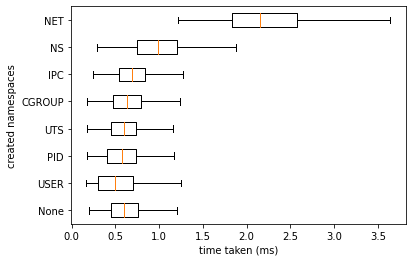
\includegraphics[width=0.7\textwidth]{graphs/namespace_times.png}

    \caption{Performance of making the \texttt{clone(2)} system call with varying namespace creation flags. The test is run in a tight compiled C loop with high precision timings taken before and after each new process is cloned and waited for. \texttt{clone(2)} presents very noisy results on a system with background activity.}
    \label{fig:namespace-times}
\end{figure}

\begin{figure}
    \centering
    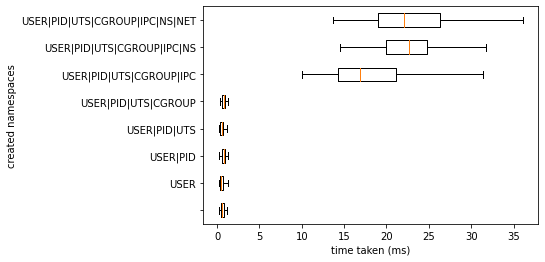
\includegraphics[width=0.8\textwidth]{graphs/namespace_stacked_times.png}

    \caption{Performance of making the \texttt{clone(2)} system call with increasing amounts of namespace creation flags. The effects of Figure \ref{fig:namespace-times} are amplified when creating multiple namespaces in a single call this frequently. There is a clear divide between the time taken for user, pid, uts, and cgroup namespaces and ipc, ns and net namespaces.}
    \label{fig:namespace-stacked-times}
\end{figure}

\begin{figure}
    \centering
    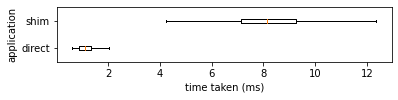
\includegraphics[width=0.8\textwidth]{graphs/fib_launch_times.png}

    \caption{A box plot comparing the performance of the Fibonacci example (§\ref{sec:building-fib} under the shim and called directly. The median time to run under the shim is approximately 800\% the time without. The inter-quartile range and range of results is also much larger.}
    \label{fig:fib-launch-times}
\end{figure}

\section{Runtime impact}
\label{sec:evaluation-runtime}

\begin{figure}
    \centering
    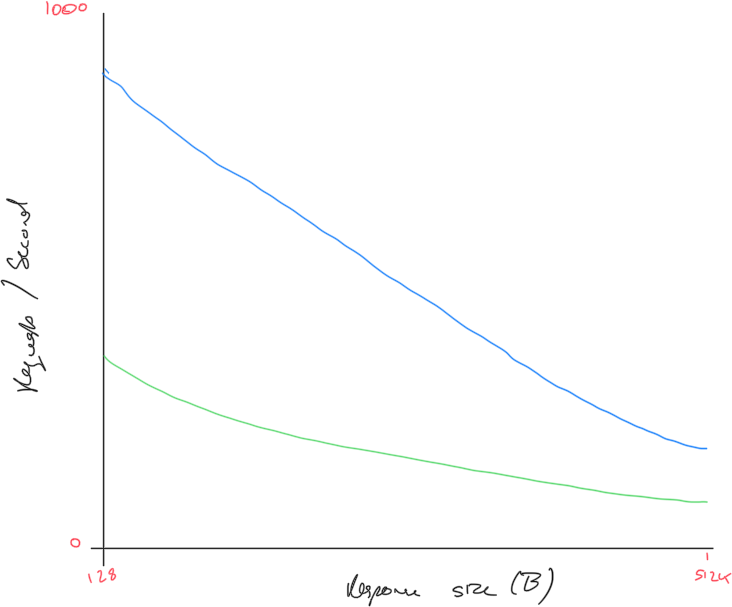
\includegraphics[width=0.8\textwidth]{graphs/tls-server-requests-per-second.png}

    \caption{\texttt{a2bench} requests per second results over 10 seconds with 100 simultaneous requests on varying response sizes. As the response size increases, the gap between the \texttt{apache2} TLS web server and the void process TLS web server decreases.}
    \label{fig:tls-performance}
\end{figure}

\section{Summary}

\todo{Evaluation: summary.}


\chapter{Conclusions}
\label{chap:conclusions}

The system built in this project enables running applications with minimal privilege in a Linux environment in a novel way. Performance is shown to be comparable, and demonstrates where the existing kernel setup provides inadequate performance for such applications. Design choices in the user-space kernel APIs for namespaces are discussed and contextualised, with suggestions offered for alternate designs.

Void processes offer a new paradigm for application development which prioritises privilege separation above all else. Rather than focusing on limiting backward compatibility, applications often need to be completely rewritten in order to take advantage of improved isolation. The system is designed to support effective static analysis on applications, though this is not implemented at this stage.

Finally, void processes provide a seamless experience without making kernel level changes, allowing for ease of deployment. Moreover, it runs on the Linux kernel, a production kernel and not a research kernel. Although the current kernel structure limits the performance of the work with namespace creation being the bottleneck, the feasibility of namespaces for process isolation is effectively demonstrated in a system that encourages application writers to develop with privilege separation as a first principle.

\section{Future Work}
\label{sec:future-work}

\subsection{Kernel API improvements}
\label{sec:future-work-kernel-api}

The primary future work to increase the utility of void processes is better performance when creating empty namespaces. Section \ref{sec:evaluation-startup} showed that the startup hit when creating the namespaces for a void is very high. This shows a limitation of the APIs, as creating a namespace that has no relation to a parent should involve a small amount of work. Secondly, an API similar to network namespaces adding paired interfaces between namespaces should be added for binding in mount namespaces, allowing mount namespaces to also be created completely empty. This would also benefit containers which by default have no connection to the parent namespace, but need to mount in their own root filesystem.

\subsection{Dynamic linking}
\label{sec:future-work-dynamic-linking}

Dynamic linking works correctly under the shim, however, it currently requires a high level of manual and static input. If one assumes trust of the binary as well as the specification, it is feasible to add a pre-spawning phase which appends read-only libraries to the specification for each spawned process automatically before creating appropriate voids. This would allow anything which can link correctly on the host system to link correctly in void processes with no additional effort.

\subsection{Building specifications from code}
\label{sec:future-work-macros}

Much of the information given in the specification and the code is shared. For example, the specification may list the arguments and also imply their type. This means that a function signature for an entrypoint implies almost all of the specification of an entrypoint, which would allow effective code generation with some supplementary information. This would remove many of the boilerplate argument processing lines from the examples and increase the usability of the system. Combining this with the dynamic linking work (§\ref{sec:future-work-dynamic-linking}) would remove a huge amount of the manual effort in creating the specification, making the system more user friendly.

\subsection{Dynamic requests}

A system for dynamically requesting statically specified network sockets was presented (§\ref{sec:filling-net}). This system of requests back to the shim could be extended to more dynamic behaviour for software that requires it. Some software, particularly that which interfaces with the user, is not able to statically specify its requirements before starting. By specifying instead a range of requests which are legal then making them dynamically, void processes would be able to support more software.

\label{lastcontentpage} % end page count here
%TC:ignore              % end word count here

\bibliographystyle{PhDbiblio-url} 
\bibliography{references}

\appendix

\label{lastpage}
%TC:endignore
\end{document}
